% Add your research tags below (comma-separated, case-insensitive)
% Year is automatically added as a tag
% <TAGs>: 2025, figures-test, neural-networks, experiments, visualization

\documentclass[11pt,letterpaper]{article}

\newcommand{\workingDate}{\textsc{2025 $|$ September $|$ 20}}
\newcommand{\userName}{Research Student}
\newcommand{\institution}{University} 

\usepackage{diary_base}
\usepackage{diary_math}

\begin{document}
\href{run:2025-09-20-figures-test.tex}{\Huge September 20} %##@@TitleDateString@@##

\section{Research with Figures}

Today's work involved analyzing several key visualizations and network architectures.

\subsection{Network Architecture}
The proposed neural network architecture is shown below:

\begin{figure}[h]
\centering
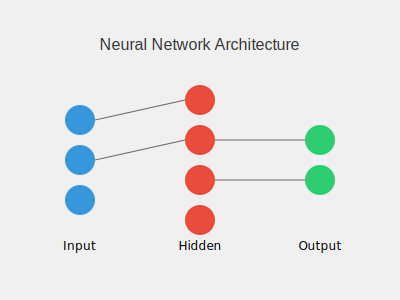
\includegraphics[width=0.8\textwidth]{figures/network_architecture.svg}
\caption{Neural network architecture overview (placeholder)}
\label{fig:network}
\end{figure}

The architecture demonstrates the flow from input layer through hidden layers to the output.

\subsection{Experimental Results}
Our experimental results are summarized in the following visualization:

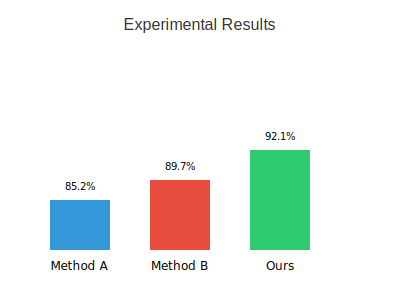
\includegraphics[width=0.6\textwidth]{figures/results_chart.svg}

The figure clearly shows the improvement in performance over baseline methods.

\subsection{Key Findings}
\begin{itemize}
\item Method C (our approach) achieved 92.1\% accuracy
\item Significant improvement over baseline methods
\item Network architecture is scalable and efficient
\end{itemize}

\bibliographystyle{apalike} 
\bibliography{reference}%##@@BibFileString@@##
\end{document}
